%%%%%%%%%%%%%%%%%%%%%%%%%%%%%%%%%%%%%%%%%%%%%%%%%%%%%%%%%%%%%%%%%%%%%%%%%%%%%%%%%%
\begin{frame}[fragile]\frametitle{}
\begin{center}
{\Large Instructions}
\end{center}
\end{frame}

%%%%%%%%%%%%%%%%%%%%%%%%%%%%%%%%%%%%%%%%%%%%%%%%%%%%%%%%%%%%%%%%%%%%%%%%%%%%%%%%%%
\begin{frame}[fragile]\frametitle{Setting Up the Environment}
    \begin{itemize}
        \item \textbf{Room Requirements:}
        \begin{itemize}
            \item Quiet, peaceful space
            \item Comfortable temperature
            \item Dim lighting
            \item No distractions (phone on silent)
        \end{itemize}
        \item \textbf{Best Practice Times:}
        \begin{itemize}
            \item Not immediately after meals
            \item Early morning or before bed
            \item Consistent practice time
        \end{itemize}
    \end{itemize}
\end{frame}

%%%%%%%%%%%%%%%%%%%%%%%%%%%%%%%%%%%%%%%%%%%%%%%%%%%%%%%%%%%%%%%%%%%%%%%%%%%%%%%%%%
\begin{frame}[fragile]\frametitle{Props and Session Duration}
    \begin{itemize}
        \item \textbf{Recommended Props:}
        \begin{itemize}
            \item Yoga mat or comfortable surface
            \item Bolster or pillow under knees
            \item Blanket for warmth
            \item Eye pillow (optional)
        \end{itemize}
        \item \textbf{Session Duration:}
        \begin{itemize}
            \item Beginners: 20-30 minutes
            \item Experienced: Up to 60 minutes
            \item Regular practice: 1-3 times per week
        \end{itemize}
    \end{itemize}
\end{frame}

%%%%%%%%%%%%%%%%%%%%%%%%%%%%%%%%%%%%%%%%%%%%%%%%%%%%%%%%%%%%%%%%%%%%%%%%%%%%%%%%%%
\begin{frame}[fragile]\frametitle{Preparation}
    \begin{itemize}
        \item Lie in Shavasana (शवासन).
        \item Bring your awareness to the space between your body and the earth.
        \item Let your body soften and sink into the floor.    
	\end{itemize}
	
      \begin{center}
        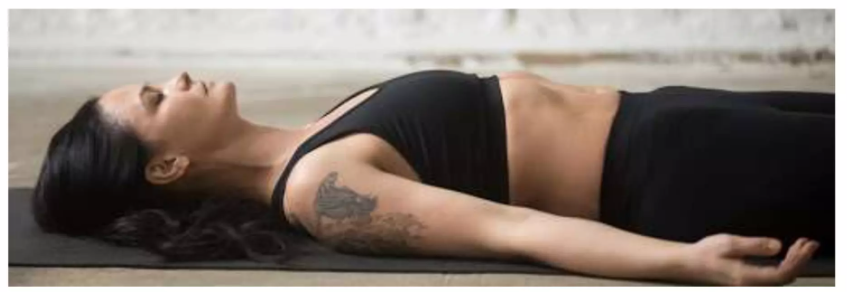
\includegraphics[width=0.8\linewidth,keepaspectratio]{yoganidra7}

		{\tiny (Ref: Yoga Nidra - Dr Amit Chail)}		
        \end{center}	
\end{frame}

%%%%%%%%%%%%%%%%%%%%%%%%%%%%%%%%%%%%%%%%%%%%%%%%%%%%%%%%%%%%%%%%%%%%%%%%%%%%%%%%%%
\begin{frame}[fragile]\frametitle{Setting the Sankalpa (संकल्प)}
    \begin{itemize}
        \item A positive “I am” statement to guide your Yoganidra practice.
        \item Examples:
        \begin{itemize}
            \item "I am strong."
            \item "I am peaceful."
            \item "I am the witness."
        \end{itemize}
        \item Repeat the Sankalpa 3 times at the start and end of Yoganidra.
    \end{itemize}
\end{frame}

%%%%%%%%%%%%%%%%%%%%%%%%%%%%%%%%%%%%%%%%%%%%%%%%%%%%%%%%%%%%%%%%%%%%%%%%%%%%%%%%%%
\begin{frame}[fragile]\frametitle{Rotation of Awareness (Abbreviated)}
    \textbf{Focus on body parts:}

\begin{columns}
    \begin{column}[T]{0.3\linewidth}
    \begin{itemize}
        \item Right heel
        \item Left heel
        \item Right calf
        \item Left calf
        \item Right knee
        \item Left knee
        \item Right thigh
        \item Left thigh
        \item Both hips
        \item Lower back
        \item Upper back
        \item Right shoulder
        \item Left shoulder
        \item Back of the head
    \end{itemize}

    \end{column}
    \begin{column}[T]{0.7\linewidth}
	      \begin{center}
        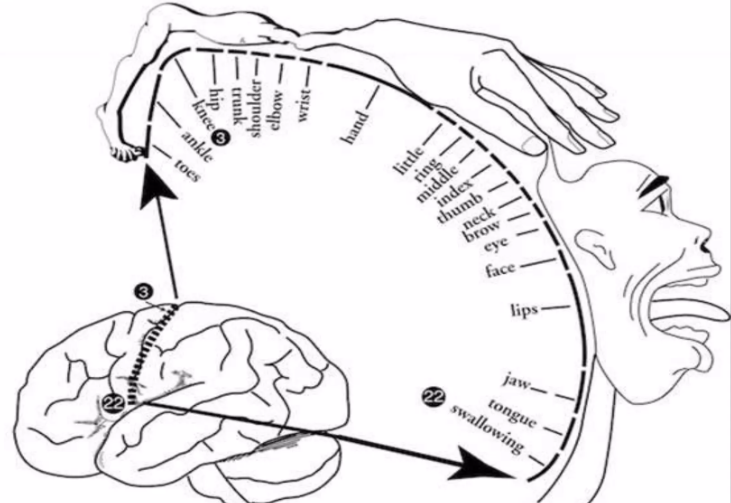
\includegraphics[width=\linewidth,keepaspectratio]{yoganidra8}

		{\tiny (Ref: Yoga Nidra - Dr Amit Chail)}		
        \end{center}
    \end{column}
  \end{columns}
  
  

	
	
\end{frame}

%%%%%%%%%%%%%%%%%%%%%%%%%%%%%%%%%%%%%%%%%%%%%%%%%%%%%%%%%%%%%%%%%%%%%%%%%%%%%%%%%%
\begin{frame}[fragile]\frametitle{Breath Awareness Techniques}
    \textbf{Progressive Breath Work:}
    \begin{itemize}
        \item Place right hand on belly, left hand on chest
        \item Observe natural breath pattern
        \item Make breath bigger gradually:
        \begin{itemize}
            \item Feel belly rise first
            \item Then chest expansion
            \item Hold briefly
            \item Release with gravity
        \end{itemize}
        \item Count breaths backwards from 27
        \item Visualize breath as golden light
    \end{itemize}
\end{frame}

%%%%%%%%%%%%%%%%%%%%%%%%%%%%%%%%%%%%%%%%%%%%%%%%%%%%%%%%%%%%%%%%%%%%%%%%%%%%%%%%%%
\begin{frame}[fragile]\frametitle{Opposite Sensations}
    \begin{itemize}
        \item Bring awareness to the sensation of heat
        \item Feel your whole body becoming warm.
        \item Shift awareness to cold. Feel the entire body cooling down.
        \item Release both sensations.
		\item Similarly: heaviness and lightness, pain and pleasure, love and hate, etc
    \end{itemize}
\end{frame}

%%%%%%%%%%%%%%%%%%%%%%%%%%%%%%%%%%%%%%%%%%%%%%%%%%%%%%%%%%%%%%%%%%%%%%%%%%%%%%%%%%
\begin{frame}[fragile]\frametitle{Guided Imagery}
    \textbf{Journey through Nature:}
    \begin{itemize}
        \item Imagine standing in a meadow, surrounded by a lush forest.
        \item Feel the warmth of the sun and smell the wildflowers.
        \item Walk into the forest, following a path that leads uphill.
        \item Reach a cave and discover a lit candle inside.
        \item Meditate on the candle's flame, with your Sankalpa inscribed on it.
    \end{itemize}
\end{frame}

%%%%%%%%%%%%%%%%%%%%%%%%%%%%%%%%%%%%%%%%%%%%%%%%%%%%%%%%%%%%%%%%%%%%%%%%%%%%%%%%%%
\begin{frame}[fragile]\frametitle{Exiting the Practice}
    \begin{itemize}
        \item Repeat your Sankalpa 3 times.
        \item Bring awareness to the sounds around you.
        \item Slowly move and break Shavasana.
    \end{itemize}
\end{frame}

%%%%%%%%%%%%%%%%%%%%%%%%%%%%%%%%%%%%%%%%%%%%%%%%%%%%%%%%%%%%%%%%%%%%%%%%%%%%%%%%%%
\begin{frame}[fragile]\frametitle{Post-Practice Reflection}
    \textbf{Journaling Guidelines:}
    \begin{itemize}
        \item Record your experience immediately after practice
        \item Note any physical sensations experienced
        \item Document emotional states encountered
        \item Track progress over time
        \item Record any insights or revelations
        \item Compare experiences across different sessions
    \end{itemize}
    \small{This reflection helps deepen your practice and track your progress.}
\end{frame}

%%%%%%%%%%%%%%%%%%%%%%%%%%%%%%%%%%%%%%%%%%%%%%%%%%%%%%%%%%%%%%%%%%%%%%%%%%%%%%%%%%
\begin{frame}[fragile]\frametitle{Best Practices for Teachers}
    \begin{itemize}
        \item \textbf{Voice and Delivery:}
        \begin{itemize}
            \item Speak in a soothing, even tone
            \item Maintain consistent pace
            \item Use clear, simple language
            \item Allow adequate pauses
        \end{itemize}
        \item \textbf{Session Management:}
        \begin{itemize}
            \item Start with shorter sessions (20-30 minutes)
            \item Progress gradually to longer sessions
            \item Always complete all stages
            \item Monitor student comfort
        \end{itemize}
    \end{itemize}
\end{frame}

%%%%%%%%%%%%%%%%%%%%%%%%%%%%%%%%%%%%%%%%%%%%%%%%%%%%%%%%%%%%%%%%%%%%%%%%%%%%%%%%%%
\begin{frame}[fragile]\frametitle{Children's Practice Considerations}
    \begin{itemize}
        \item \textbf{Session Duration:}
        \begin{itemize}
            \item Keep sessions shorter (10-15 minutes)
            \item Use age-appropriate language
            \item Include playful visualization
        \end{itemize}
        \item \textbf{Special Elements:}
        \begin{itemize}
            \item Use simple counting exercises (40 to 1)
            \item Include light visualization exercises
            \item Incorporate gentle encouragement
            \item Allow natural breaks in concentration
        \end{itemize}
        \item \textbf{Closing Practice:}
        \begin{itemize}
            \item End with positive affirmations
            \item Include sharing of "light" with loved ones
            \item Gentle return to regular awareness
        \end{itemize}
    \end{itemize}
\end{frame}